% AREA OF IRREGULAR POLYGONS - WORKSHEET 0
\documentclass[12pt, letterpaper, fleqn]{article}

% ----------------------------------------------------------
% PACKAGES
% ----------------------------------------------------------
\usepackage{graphicx}
\usepackage{xcolor}
\usepackage[most]{tcolorbox}
\usepackage{amsmath, amssymb}
\usepackage{fancyhdr}
\usepackage[utf8]{inputenc}
\usepackage[T1]{fontenc}
\usepackage{enumitem}
\usepackage{geometry}
\usepackage{tikz}
\usepackage{needspace}
\usepackage{multicol}

\usetikzlibrary{arrows.meta, calc}

% ----------------------------------------------------------
% PAGE SETUP
% ----------------------------------------------------------
\usepackage{times}
\geometry{letterpaper, top=1.25in, bottom=1.25in, marginpar=0.5in}

% ----------------------------------------------------------
% HEADER / FOOTER
% ----------------------------------------------------------
\newcommand{\logowidth}{3cm}
\setlength{\headheight}{20pt}
\setlength{\footskip}{40pt}

\pagestyle{fancy}
\fancyhf{}
\fancyhead[C]{\small\bfseries Area of Irregular Polygons}
\fancyfoot[L]{\raisebox{2pt}{
\includegraphics[width=\logowidth]{kss.png}}}
\fancyfoot[C]{\thepage}
\fancyfoot[R]{6.17.0}

\renewcommand{\footrulewidth}{0.2pt}

% ----------------------------------------------------------
% HELPER MACROS
% ----------------------------------------------------------
\newcommand{\blank}{\underline{\hspace{2.2cm}}}
\newcommand{\blanklong}{\underline{\hspace{6.5cm}}}
\newcommand{\blankshorter}{\underline{\hspace{1.5cm}}}

% ----------------------------------------------------------
% DOCUMENT
% ----------------------------------------------------------
\begin{document}


% ==========================================================
% WORKSHEET 0: FOUNDATION
% ==========================================================
\pagestyle{fancy}
\fancyhf{}
\fancyhead[C]{\small\bfseries Area of Irregular Polygons --- Worksheet 0}
\fancyfoot[C]{\thepage}
\fancyfoot[R]{6.17.0}
\renewcommand{\footrulewidth}{0.2pt}

\textbf{Name:} \underline{\hspace{5cm}} \hfill \textbf{Date:} \underline{\hspace{3cm}}\\

\begin{tcolorbox}[colback=black!10]
    \large\textcolor{black}{\textbf{Area of Irregular and Composite Polygons (Foundation)}}
\end{tcolorbox}

\vspace{2mm}
\noindent
1. \textbf{Decomposition:} Break down complex shapes into simpler pieces (rectangles, triangles) and sum their areas. \\
2. \textbf{Subtraction Method:} Draw a bounding box around the shape, find its area, and subtract empty sections. \\
3. \textbf{Coordinate Grid Polygons:} Calculate side lengths by finding horizontal and vertical distance: $\text{Distance} = |x_2 - x_1|$ or $|y_2 - y_1|$.

\vspace{3mm}

% --- STRATEGY DIAGRAM VISUAL SCAFFOLD ---
\begin{center}
\begin{tikzpicture}[scale=0.8, every node/.style={transform shape}]
    % Left Box: Decomposition
    \draw[thick, fill=blue!5] (0,0) rectangle (2.5,2);
    \draw[thick, dashed, red] (1,0) -- (1,2);
    \node at (0.5,1) {$A_1$}; \node at (1.75,1) {$A_2$};
    \node[below] at (1.25,-0.1) {\textbf{Decompose ($A_1 + A_2$)}};

    % Right Box: Subtraction
    \draw[thick, fill=green!5] (5,0) -- (7.5,0) -- (7.5,1.2) -- (6.3,1.2) -- (6.3,2) -- (5,2) -- cycle;
    \draw[thick, red, dashed] (6.3,1.2) rectangle (7.5,2);
    \node at (5.8,1) {Solid}; \node[red] at (6.9,1.6) {\small Cut};
    \node[below] at (6.25,-0.1) {\textbf{Subtract ($\text{Total} - \text{Cut}$)}};
\end{tikzpicture}
\end{center}

\vspace{2mm}

\begin{tcolorbox}[colback=white, colframe=black!25, boxrule=0.6pt, arc=4mm, left=6mm, right=6mm, top=4mm, bottom=4mm]
\textbf{Worked Example 1A: Decomposition via Split}

\medskip
\noindent
An L-shaped polygon has a height of 10 cm and a total width of 8 cm. Its vertical column is 4 cm wide, and the horizontal base is 3 cm high. Find its area.\\
\textbf{Solution:} \\
1) Decompose vertically: Left block width is $4\text{ cm}$, height is $10 - 3 = 7\text{ cm}$. $\text{Area}_1 = 4 \times 7 = 28\text{ cm}^2$.\\
2) Horizontal base piece: Width is $8\text{ cm}$, height is $3\text{ cm}$. $\text{Area}_2 = 8 \times 3 = 24\text{ cm}^2$.\\
3) Total Sum: $\text{Total Area} = 28 + 24 = 52\text{ cm}^2$.
\end{tcolorbox}

\vspace{3mm}

\begin{tcolorbox}[colback=white, colframe=black!25, boxrule=0.6pt, arc=4mm, left=6mm, right=6mm, top=4mm, bottom=4mm]
\textbf{Worked Example 1B: Coordinate Length Processing}

\medskip
\noindent
\textbf{Problem:} Find the side lengths and area of a rectangle with vertices at $(2, 3)$, $(7, 3)$, $(7, 8)$, and $(2, 8)$.

\medskip
\noindent
\textbf{Solution:} \\
1) Horizontal Base length: Subtract $x$-coordinates $\implies |7 - 2| = 5\text{ units}$.\\
2) Vertical Height length: Subtract $y$-coordinates $\implies |8 - 3| = 5\text{ units}$.\\
3) Calculate Area: $\text{Area} = \text{base} \times \text{height} = 5 \times 5 = 25\text{ sq units}$.
\end{tcolorbox}

\newpage

\begin{tcolorbox}[colback=white, colframe=black!25, boxrule=0.6pt, arc=4mm, left=6mm, right=6mm, top=4mm, bottom=4mm]
\textbf{Worked Example 1C: 3D Wall Lateral Area Conversions}

\medskip
\noindent
\textbf{Problem:} A room floor plan layout has a total wall perimeter of 40 feet. The room has 8-foot high ceilings. If a door cutout takes up $21\text{ ft}^2$, find the total remaining wall surface area to paint.

\medskip
\noindent
\textbf{Solution:} \\
1) Find gross total wall area before exclusions:
$$\text{Gross Area} = \text{Perimeter} \times \text{Ceiling Height} = 40 \times 8 = 320\text{ ft}^2$$
2) Deduct unshaded architectural openings:
$$\text{Paintable Area} = 320 - 21 = 299\text{ ft}^2$$
\end{tcolorbox}

\vspace{4mm}

\begin{tcolorbox}[colback=white, colframe=black, boxrule=1pt, arc=4mm, left=6mm, right=6mm, top=5mm, bottom=5mm]
\textbf{Deeper Thinking Problem 1: Decomposition Methods Comparison}

\medskip
\noindent
\textbf{a)} A polygon has coordinates $A(-2, 1)$, $B(4, 1)$, $C(4, 5)$, $D(1, 5)$, $E(1, 3)$, and $F(-2, 3)$. Draw this shape, decompose it in two different ways, and show that both ways yield the same area.
\vspace{3.5cm}

\noindent
\textbf{b)} Explain how the subtraction method works for finding the area of a right triangle with vertices $X(0, 0)$, $Y(6, 0)$, and $Z(0, 4)$ using an outer bounding rectangle.
\vspace{3.5cm}
\end{tcolorbox}

\begin{tcolorbox}[colback=white, colframe=black, boxrule=1pt, arc=4mm, left=6mm, right=6mm, top=5mm, bottom=5mm]
\textbf{Deeper Thinking Problem 2: Irregular Shapes in Context}

\medskip
\noindent
\textbf{a)} A classroom is shaped like a large rectangle ($15\text{ ft} \times 20\text{ ft}$) with an additional rectangular recess ($5\text{ ft} \times 8\text{ ft}$) on one side. What is the total area of the floor? Show your division layout.
\vspace{3.5cm}

\noindent
\textbf{b)} Find the area of a shaded region inside a $12\text{ cm} \times 12\text{ cm}$ square if there is an unshaded central square of $4\text{ cm} \times 4\text{ cm}$ cleanly cut out.
\vspace{3.5cm}
\end{tcolorbox}


\begin{tcolorbox}[colback=white, colframe=black, boxrule=1pt, arc=4mm, left=6mm, right=6mm, top=5mm, bottom=5mm]
\textbf{Deeper Thinking Problem 3: Composite Figures and Area}

\medskip
\noindent
\textbf{a)} A composite figure is made of a rectangle ($8\text{ m} \times 5\text{ m}$) with a right triangle ($\text{base} = 5\text{ m}$, $\text{height} = 4\text{ m}$) attached to its right side. Calculate the total area.
\vspace{3cm}

\noindent
\textbf{b)} An H-shaped figure has two vertical rectangles ($3\text{ in} \times 10\text{ in}$ each) connected by a horizontal bridge ($6\text{ in} \times 2\text{ in}$). Find the total area.
\vspace{3cm}

\end{tcolorbox}

\newpage

\begin{tcolorbox}[colback=white, colframe=black, boxrule=1pt, arc=4mm, left=6mm, right=6mm, top=5mm, bottom=5mm]
\textbf{Deeper Thinking Problem 4: Real-World Design Problem}

\medskip
\noindent
\textbf{a)} A park layout forms a composite polygon. It consists of a rectangular main area of $40\text{ m} \times 25\text{ m}$, a triangular garden in one corner with base $10\text{ m}$ and height $15\text{ m}$, and a square fountain cut out of the center ($5\text{ m} \times 5\text{ m}$). Find the total usable area of the park.
\vspace{5cm}

\noindent
\textbf{b)} If seeding the grass costs \$0.80 per square meter, how much would it cost to seed the entire usable area calculated above?
\vspace{5cm}

\noindent
\textbf{c)} Describe in words a decomposition strategy you could use for an irregular polygon that has no right angles. How do you approach finding its altitudes?
\vspace{5cm}
\end{tcolorbox}

\newpage

\end{document}
